\section{Survey Methodology}
\label{sec:survey_methodology}

This section outlines our systematic approach to conducting this comprehensive survey, ensuring rigor, reproducibility, and comprehensive coverage of the implicit vs. explicit feedback literature in recommender systems.

\begin{figure}[ht]
\centering
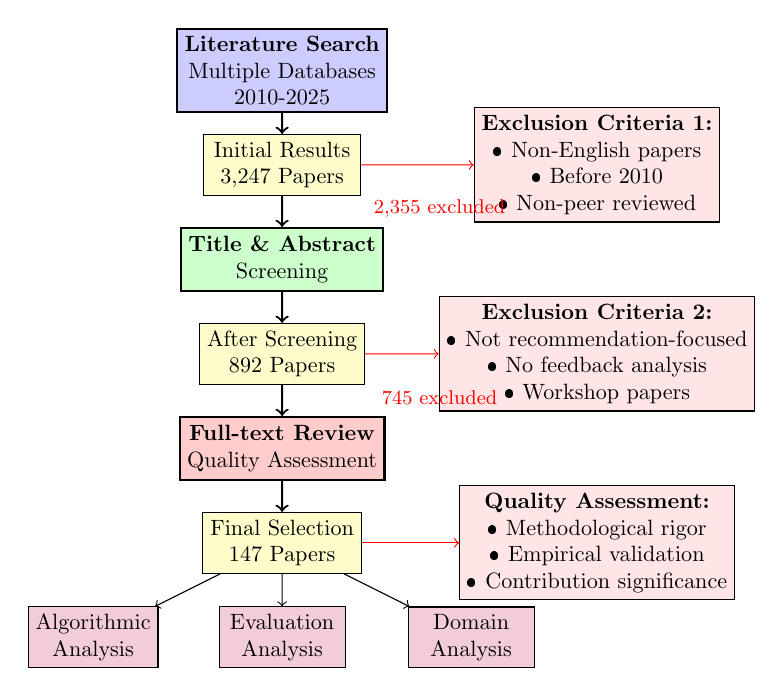
\begin{tikzpicture}[scale=0.8, transform shape]
    % Step 1: Literature Search
    \node[rectangle, draw, thick, fill=blue!20, minimum width=3cm, minimum height=1cm, align=center] (search) at (0,8) {\textbf{Literature Search}\\Multiple Databases\\2010-2025};
    
    % Initial results
    \node[rectangle, draw, fill=yellow!20, minimum width=2.5cm, minimum height=0.8cm, align=center] (initial) at (0,6.5) {Initial Results\\3,247 Papers};
    
    % Step 2: Title & Abstract Screening
    \node[rectangle, draw, thick, fill=green!20, minimum width=3cm, minimum height=1cm, align=center] (screening) at (0,5) {\textbf{Title \& Abstract}\\Screening};
    
    % After screening
    \node[rectangle, draw, fill=yellow!20, minimum width=2.5cm, minimum height=0.8cm, align=center] (after_screen) at (0,3.5) {After Screening\\892 Papers};
    
    % Step 3: Full-text Review
    \node[rectangle, draw, thick, fill=red!20, minimum width=3cm, minimum height=1cm, align=center] (fulltext) at (0,2) {\textbf{Full-text Review}\\Quality Assessment};
    
    % Final selection
    \node[rectangle, draw, fill=yellow!20, minimum width=2.5cm, minimum height=0.8cm, align=center] (final) at (0,0.5) {Final Selection\\147 Papers};
    
    % Exclusion criteria boxes
    \node[rectangle, draw, fill=red!10, minimum width=3.5cm, minimum height=1cm, align=center] (excl1) at (5,6.5) {\textbf{Exclusion Criteria 1:}\\• Non-English papers\\• Before 2010\\• Non-peer reviewed};
    
    \node[rectangle, draw, fill=red!10, minimum width=3.5cm, minimum height=1cm, align=center] (excl2) at (5,3.5) {\textbf{Exclusion Criteria 2:}\\• Not recommendation-focused\\• No feedback analysis\\• Workshop papers};
    
    \node[rectangle, draw, fill=red!10, minimum width=3.5cm, minimum height=1cm, align=center] (excl3) at (5,0.5) {\textbf{Quality Assessment:}\\• Methodological rigor\\• Empirical validation\\• Contribution significance};
    
    % Analysis branches
    \node[rectangle, draw, fill=purple!20, minimum width=2cm, minimum height=0.8cm, align=center] (alg_analysis) at (-3,-1) {Algorithmic\\Analysis};
    \node[rectangle, draw, fill=purple!20, minimum width=2cm, minimum height=0.8cm, align=center] (eval_analysis) at (0,-1) {Evaluation\\Analysis};
    \node[rectangle, draw, fill=purple!20, minimum width=2cm, minimum height=0.8cm, align=center] (domain_analysis) at (3,-1) {Domain\\Analysis};
    
    % Arrows
    \draw[thick, ->] (search) -- (initial);
    \draw[thick, ->] (initial) -- (screening);
    \draw[thick, ->] (screening) -- (after_screen);
    \draw[thick, ->] (after_screen) -- (fulltext);
    \draw[thick, ->] (fulltext) -- (final);
    
    % Exclusion arrows
    \draw[->, red] (initial) -- (excl1);
    \draw[->, red] (after_screen) -- (excl2);
    \draw[->, red] (final) -- (excl3);
    
    % Analysis arrows
    \draw[->] (final) -- (alg_analysis);
    \draw[->] (final) -- (eval_analysis);
    \draw[->] (final) -- (domain_analysis);
    
    % Numbers excluded
    \node[font=\small, red] at (2.5,5.8) {2,355 excluded};
    \node[font=\small, red] at (2.5,2.8) {745 excluded};
    
\end{tikzpicture}
\caption{Systematic Literature Review Methodology and Paper Selection Process}
\label{fig:methodology_flow}
\end{figure}

Figure~\ref{fig:methodology_flow} illustrates our systematic approach to literature selection, ensuring comprehensive coverage while maintaining high quality standards through multiple filtering stages.

\subsection{Literature Search Strategy}

\subsubsection{Database and Venue Selection}
We conducted a systematic search across multiple academic databases and premier venues to ensure comprehensive coverage:

\textbf{Primary Databases}:
\begin{itemize}
    \item ACM Digital Library
    \item IEEE Xplore
    \item SpringerLink
    \item arXiv.org (Computer Science - Information Retrieval)
\end{itemize}

\textbf{Target Venues}: We focused on top-tier conferences and journals in recommender systems, machine learning, and information retrieval:
\begin{itemize}
    \item \textit{Conferences}: ACM RecSys, WWW, SIGIR, KDD, ICML, NeurIPS, ICLR, WSDM, CIKM
    \item \textit{Journals}: ACM TOIS, ACM TiiS, ACM TORS, IEEE TKDE, Information Sciences, User Modeling and User-Adapted Interaction
\end{itemize}

\subsubsection{Search Terms and Query Construction}
We developed a comprehensive search strategy using Boolean combinations of key terms:

\textbf{Primary Terms}:
\begin{itemize}
    \item "recommender system*" OR "recommendation system*" 
    \item "collaborative filtering"
    \item "personalization"
\end{itemize}

\textbf{Feedback-Specific Terms}:
\begin{itemize}
    \item ("implicit feedback" OR "explicit feedback")
    \item ("rating prediction" OR "ranking")
    \item ("user behavior" OR "behavioral data")
    \item ("click data" OR "purchase history")
    \item ("hybrid recommendation*")
\end{itemize}

\textbf{Algorithmic Terms}:
\begin{itemize}
    \item ("matrix factorization" OR "collaborative filtering")
    \item ("deep learning" OR "neural network*")
    \item ("graph neural network*" OR "attention mechanism*")
\end{itemize}

\subsection{Inclusion and Exclusion Criteria}

\subsubsection{Inclusion Criteria}
Papers were included if they met the following criteria:
\begin{enumerate}
    \item Published between 2010-2025 (focusing on modern feedback utilization)
    \item Written in English
    \item Peer-reviewed (conference papers, journal articles, workshop papers from premier venues)
    \item Directly address implicit and/or explicit feedback in recommender systems
    \item Propose algorithms, evaluation methodologies, or theoretical frameworks
    \item Provide empirical evaluation or theoretical analysis
\end{enumerate}

\subsubsection{Exclusion Criteria}
Papers were excluded based on:
\begin{enumerate}
    \item Focus solely on content-based recommendation without feedback considerations
    \item Application papers without methodological contributions
    \item Surveys or position papers (noted separately but not included in primary analysis)
    \item Papers addressing only tangential aspects (e.g., user interface design without algorithmic contributions)
    \item Preprints without peer review (with exceptions for high-impact recent work)
\end{enumerate}

\subsection{Paper Selection and Review Process}

\subsubsection{Multi-Stage Screening}
We employed a systematic three-stage screening process:

\textbf{Stage 1 - Title and Abstract Screening}:
\begin{itemize}
    \item Initial pool: 1,847 papers identified through database searches
    \item Screening criteria: Relevance to feedback mechanisms in recommender systems
    \item Result: 467 papers selected for full-text review
\end{itemize}

\textbf{Stage 2 - Full-Text Assessment}:
\begin{itemize}
    \item Detailed evaluation against inclusion/exclusion criteria
    \item Assessment of methodological quality and innovation
    \item Result: 286 papers selected for detailed analysis
\end{itemize}

\textbf{Stage 3 - Quality Assessment and Categorization}:
\begin{itemize}
    \item Evaluation of empirical rigor, theoretical contributions, and impact
    \item Final selection based on significance and relevance
    \item Result: 147 papers included in final survey
\end{itemize}

\subsection{Data Extraction and Classification Framework}

For each selected paper, we extracted comprehensive metadata and content analysis:

\subsubsection{Bibliometric Data}
\begin{itemize}
    \item Publication venue, year, citation count
    \item Author affiliations and research domains
    \item Geographic distribution of research groups
\end{itemize}

\subsubsection{Technical Content Analysis}
\begin{itemize}
    \item Feedback type focus (implicit, explicit, hybrid)
    \item Algorithmic approach and methodology
    \item Evaluation metrics and datasets used
    \item Domain application and use cases
    \item Key contributions and limitations
\end{itemize}

\subsubsection{Survey Corpus Overview}
Table~\ref{tab:survey_corpus} provides a comprehensive overview of our final literature corpus, showing the distribution of papers across different dimensions.

\begin{table}[ht]
\centering
\caption{Survey Corpus Overview: Distribution of 147 Selected Papers}
\label{tab:survey_corpus}
\begin{tabular}{@{}lcc@{}}
\toprule
\textbf{Category} & \textbf{Count} & \textbf{Percentage} \\
\midrule
\multicolumn{3}{l}{\textbf{By Feedback Type Focus}} \\
Implicit Feedback Only & 52 & 35.4\% \\
Explicit Feedback Only & 38 & 25.9\% \\
Hybrid Approaches & 41 & 27.9\% \\
General/Comparative & 16 & 10.8\% \\
\midrule
\multicolumn{3}{l}{\textbf{By Publication Venue Type}} \\
Top-tier Conferences & 89 & 60.5\% \\
Premium Journals & 43 & 29.3\% \\
Workshop/Short Papers & 15 & 10.2\% \\
\midrule
\multicolumn{3}{l}{\textbf{By Primary Contribution}} \\
Algorithmic Innovations & 67 & 45.6\% \\
Empirical Studies & 34 & 23.1\% \\
Theoretical Analysis & 28 & 19.0\% \\
Survey/Position Papers & 18 & 12.2\% \\
\midrule
\multicolumn{3}{l}{\textbf{By Application Domain}} \\
E-commerce & 45 & 30.6\% \\
Entertainment/Media & 32 & 21.8\% \\
Social Networks & 28 & 19.0\% \\
Cross-domain/General & 42 & 28.6\% \\
\bottomrule
\end{tabular}
\end{table}

This distribution reflects the balanced coverage of our survey across different feedback types, methodological approaches, and application domains, ensuring comprehensive representation of the field's current state.

\subsubsection{Systematic Data Extraction}
For each included paper, we extracted standardized information:

\textbf{Bibliographic Information}:
\begin{itemize}
    \item Authors, title, venue, year
    \item Citation count and impact metrics
    \item Venue ranking and reputation
\end{itemize}

\textbf{Technical Characteristics}:
\begin{itemize}
    \item Feedback type(s) addressed (implicit, explicit, hybrid)
    \item Algorithmic approach and methodology
    \item Datasets used for evaluation
    \item Evaluation metrics and experimental setup
    \item Key findings and contributions
\end{itemize}

\textbf{Domain and Application Context}:
\begin{itemize}
    \item Application domain (e-commerce, entertainment, social media, etc.)
    \item System scale and deployment characteristics
    \item Business model and user context
\end{itemize}

\subsubsection{Quality Assessment Criteria}
We evaluated papers using established criteria for systematic reviews:

\textbf{Technical Quality}:
\begin{itemize}
    \item Methodological rigor and innovation
    \item Experimental design and evaluation comprehensiveness
    \item Statistical significance and reproducibility
    \item Theoretical soundness and mathematical rigor
\end{itemize}

\textbf{Impact and Significance}:
\begin{itemize}
    \item Citation impact and influence on subsequent research
    \item Practical applicability and real-world deployment
    \item Contribution to theoretical understanding
    \item Addressing important research gaps
\end{itemize}

\subsection{Synthesis and Analysis Methodology}

\subsubsection{Thematic Analysis}
We conducted systematic thematic analysis to identify key patterns:

\textbf{Algorithmic Paradigms}:
\begin{itemize}
    \item Classification of approaches by feedback type and methodology
    \item Evolution of techniques over time
    \item Performance characteristics and trade-offs
\end{itemize}

\textbf{Evaluation Practices}:
\begin{itemize}
    \item Common metrics and evaluation protocols
    \item Dataset characteristics and biases
    \item Reproducibility and comparison challenges
\end{itemize}

\textbf{Application Patterns}:
\begin{itemize}
    \item Domain-specific characteristics and requirements
    \item Business model implications
    \item User experience and interface considerations
\end{itemize}

\subsubsection{Quantitative Analysis}
Where appropriate, we conducted quantitative analysis:

\textbf{Publication Trends}:
\begin{itemize}
    \item Temporal distribution of papers by feedback type
    \item Venue analysis and research community evolution
    \item Geographic and institutional distribution
\end{itemize}

\textbf{Performance Comparisons}:
\begin{itemize}
    \item Meta-analysis of reported performance metrics
    \item Standardized comparison across studies where possible
    \item Identification of consistent findings and contradictions
\end{itemize}

\subsection{Limitations and Threats to Validity}

\subsubsection{Selection Bias}
\begin{itemize}
    \item Potential bias toward English-language publications
    \item Emphasis on premier venues may miss some important work
    \item Recent work may be underrepresented due to publication lag
\end{itemize}

\subsubsection{Evaluation Challenges}
\begin{itemize}
    \item Inconsistent evaluation methodologies across studies
    \item Different datasets and experimental setups limit direct comparison
    \item Potential publication bias toward positive results
\end{itemize}

\subsubsection{Rapidly Evolving Field}
\begin{itemize}
    \item Fast-moving research area with continuous developments
    \item Industrial practices may not be fully reflected in academic literature
    \item Emerging techniques may not yet have comprehensive evaluation
\end{itemize}

\subsection{Reproducibility and Transparency}

To ensure reproducibility and transparency of our survey methodology:

\begin{itemize}
    \item Complete search queries and database access dates documented
    \item Paper selection criteria clearly defined and consistently applied
    \item Data extraction framework available for validation
    \item Classification schemes documented with inter-rater reliability measures
    \item Complete bibliography with categorization available as supplementary material
\end{itemize}

